\documentclass[preview]{standalone}

\usepackage{amsmath}
\usepackage{amssymb}
\usepackage{stellar}
\usepackage{definitions}
\usepackage{enumitem}
\usepackage{tikz}

\usetikzlibrary{automata,arrows}

\begin{document}

\id{linearalgebra-exercises-batch-12}
\genpage

\section{Exercises}

\begin{snippetexercise}{linear-algebra-batch-12-ex-1}{}
    Find eigenvalues and eigenvectors for the following matrices in \(\matrices_{n \times n}(\mathbb F)\)
    where \(\mathbb F = \realnumbers, \complexnumbers\):
    \[
        \begin{pmatrix}
            2 & 7 \\ 7 & 24
        \end{pmatrix},
        \quad
        \begin{pmatrix}
            1 & 1 & 1 \\ 0 & 1 & 0 \\ 1 & 1 & 1
        \end{pmatrix},
        \quad
        \begin{pmatrix}
            -11 & -24 & -18 \\ 8 & 17 & 12 \\ -2 & -4 & -2
        \end{pmatrix},
        \quad
        \begin{pmatrix}
            0 & -2 & 1 \\ 2 & -5 & 2 \\ -1 & 2 & -2
        \end{pmatrix},
        \quad
        \begin{pmatrix}
            4 & 0 & -2 & 0 \\ 0 & 2 & 0 & 5 \\ 3 & 0 & -1 & 0 \\ 0 & -1 & 0 & -2
        \end{pmatrix}
    \]
\end{snippetexercise}

\begin{snippetsolution}{linear-algebra-batch-12-ex-1-sol}{}
    \todo
\end{snippetsolution}

\begin{snippetexercise}{linear-algebra-batch-12-ex-2}{}
    Let \(V\) be a real vector space of finite dimension.
    Given two operators \(f,g \in \operatorname{End}(V)\) we know that
    \[
        f^2 = \text{Id}_V \land g^2 - 5g + 6 \text{Id}_V = 0
    \]
    where \(f^2 = f \circ f\) and \(g^2 = g \circ g\). Show that \(f\) and \(g\) are diagonalizable. 
\end{snippetexercise}

\begin{snippetsolution}{linear-algebra-batch-12-ex-2-sol}{}
    \todo
\end{snippetsolution}

\begin{snippetexercise}{linear-algebra-batch-12-ex-3}{}
    Decide whether the following matrices in
    \(\matrices_{3 \times 3}(\realnumbers)\) are diagonalizable:
    \[\begin{pmatrix} 1 & 0 & 0 \\ 0 & -1 & 1 \\ 0 & 0 & -1 \end{pmatrix}, \quad \begin{pmatrix} 1 & 0 & 1 \\ 0 & 1 & -2 \\ 0 & 0 & 2 \end{pmatrix} \quad \text{and} \quad \begin{pmatrix} 5 & 1 & -1 \\ 2 & 4 & -2 \\ 1 & -1 & 3 \end{pmatrix}.\]
    If they are, find a basis of \(\realnumbers^3\) consisting of eigenvectors.
\end{snippetexercise}

\begin{snippetsolution}{linear-algebra-batch-12-ex-3-sol}{}
    \todo
\end{snippetsolution}

\begin{snippetexercise}{linear-algebra-batch-12-ex-4}{}
    Determine for which values of the parameters \(a\) and \(b\) the \matrix
    \[A = \begin{pmatrix} 5 & 0 & 0 \\ 0 & -1 & a \\ 3 & 0 & b \end{pmatrix} \in \matrices_{3 \times 3}(\realnumbers)\] is diagonalizable.
    For such values, find a basis of \(\realnumbers^3\) consisting of eigenvectors.
\end{snippetexercise}

\begin{snippetsolution}{linear-algebra-batch-12-ex-4-sol}{}
    \todo
\end{snippetsolution}

\begin{snippetexercise}{linear-algebra-batch-12-ex-5}{}
    Let \(f \colon \rationalnumbers^3 \fromto \rationalnumbers^3\) be the linear map
    determined by \[f(7, 3, 0) = (0, 7, 3), \quad f(1, 1, 3) = (18, -32, 19) \quad \text{and} \quad f(3, 2, 4) = (24, -41, 26).\]
    Find a basis of \(\rationalnumbers^3\) consisting of eigenvectors of \(f\).
\end{snippetexercise}

\begin{snippetsolution}{linear-algebra-batch-12-ex-5-sol}{}
    \todo
\end{snippetsolution}

\begin{snippetexercise}{linear-algebra-batch-12-ex-6}{}
    Consider the \matrix
    \[A = \begin{pmatrix} \frac{5}{2} & -1 \\ 3 & -1 \end{pmatrix} \in \matrices_{2 \times 2}(\realnumbers).\]
    \begin{enumerate}[label=\Alph*]
        \item Diagonalize \(A\).
        \item Calculate \(A^{2025}\) and \(\lim_{n \to \infty} A^n\).
    \end{enumerate}
\end{snippetexercise}

\begin{snippetsolution}{linear-algebra-batch-12-ex-6-sol}{}
    \todo
\end{snippetsolution}

\begin{snippetexercise}{linear-algebra-batch-12-ex-7}{}
    A particle \(P\) can be found, at every discrete time \(t\geq 0\), in a state \(A\)
    or \(B\). The probability of \(P\) switching state are given in the following diagram:
    \begin{center}
        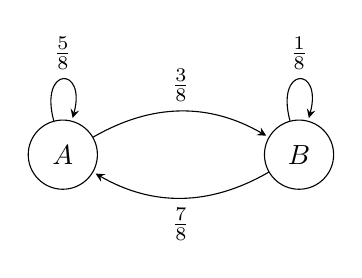
\begin{tikzpicture}[->,>=stealth,shorten >=1pt,auto,node distance=3cm]
        % nodi
        \node[state] (A)                    {$A$};
        \node[state] (B) [right of=A]      {$B$};
        % archi
        \path
            (A) edge[loop above]   node{$\tfrac{5}{8}$} (A)
                edge[bend left]    node{$\tfrac{3}{8}$} (B)
            (B) edge[loop above]   node{$\tfrac{1}{8}$} (B)
                edge[bend left]    node{$\tfrac{7}{8}$} (A);
        \end{tikzpicture}
    \end{center}
    For \(t=0\), the particle is equally likely to be in state \(A\) or \(B\). Find
    the probabilities of each state for \(t=1\) and for \(t = n\) when \(n\to\infty\).
\end{snippetexercise}

\begin{snippetsolution}{linear-algebra-batch-12-ex-7-sol}{}
    \todo
\end{snippetsolution}

\end{document}